\section{Dataset}
The depth map captured by Kinect is usually semi-dense with a number of missing pixels, as shown in Figure \ref{fig:depth_map_kinect}. Consequently, the ground truth of inferenced normal map is incomplete, either. 





\begin{figure}[!h]
	\centering
	{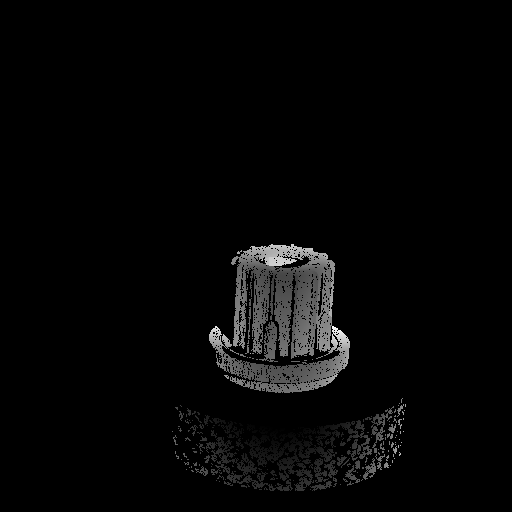
\includegraphics[width=0.4\textwidth]{./pic/00028.depth0.png}}
	\label{fig:depth_map_kinect}
	\caption{Depth Map of an object captured by Kinect}
\end{figure}

In view of this this kind of situation, a set of generated synthetic 3D scene via Unity is used as training dataset.  The main advantage using generated scene is the complete information of all the information in the synthetic world. The depth map can be captured loss-free. The corresponding normal map can also be safely considered as ground truth. To construct the dataset, 22 3D models have been used and 1000 different scenes have been captured with different pose of each model. 3 kinds of images are recorded in each scene:

\begin{itemize}
	\item Depth map
	\item Grayscale image
	\item Normal Map
\end{itemize}

\subsection{Noise}
The raw depth maps captured by Kinect usually have missing pixels. As shown in picture \ref{fig:depth_map_kinect}.
Observing the depth map, the missing pixels can be divided into two groups.
\begin{itemize}
	\item random missed single pixels
	\item missed dark areas
\end{itemize}
Since the input of evaluation is incomplete Kinect depth map, thus the input of training should have the similar pattern as well. That is, adding the similar noise to synthetic depth map.
For the two kinds of depth noise, first can be simulated by adding uniformly distributed black pixels to the whole depth map, whereas the second can be dealed with a high-pass filter to filter out dark pixels and set them to 0.

%% add noise image
\begin{figure}[!h]
	\centering
	\begin{tikzpicture}
		\node[inner sep=0pt] (depthmap) at (0,0)
		{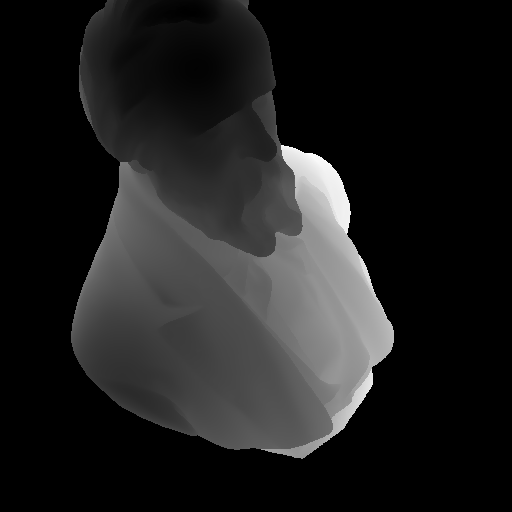
\includegraphics[width=.2\textwidth]{./pic/00440.depth0.png}};
		\draw [-stealth](2,0) -- (3,0);
		\node[inner sep=0pt] (depthmap) at (5,0)
		{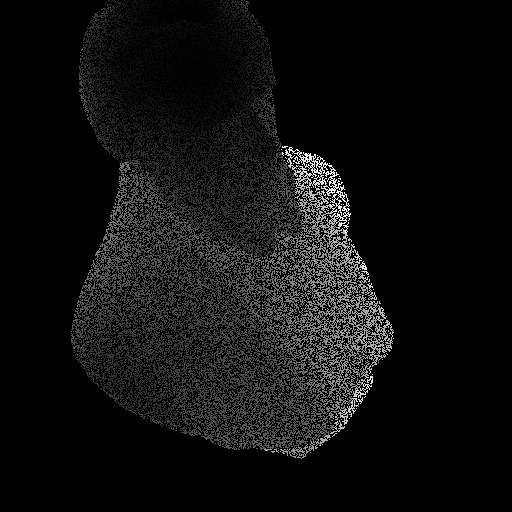
\includegraphics[width=.2\textwidth]{./pic/00440.depth0_noise.png}};
	\end{tikzpicture}
\end{figure}

Specifically, for each pixel with index $ (i,j) $ in a synthetic depth map $ D $, if its value less than a threshold $ B $, then set it to $ 0 $, i.e.
\[D(i,j) = \begin{cases}
		0 & D(i,j) \le B \\
		D(i,j) & D(i,j) > B
	\end{cases}  \]

for the rest of the pixels, the following two equal-opportunity situations will occur,
\begin{itemize}
	\item pixel value remain same
	\item pixel value set to $ 0 $
\end{itemize}


\section{Gated Convolution}

Gated Convolution layer\cite{gconv}, the output of the layer with input size $ (N, C_{in}, H, W) $ and output $ (N, C_{out}, H_{out}, W_{out}) $ can be described as:
\begin{equation}\label{gconv}
	o(N_i, C_{o_j}) = \sigma(\sum_{k=0}^{C_{in}-1}w_g(C_{o_j}, k) \star i(N_i,k) + b_g(C_{o_j})) * 
	\phi (\sum_{k=0}^{C_{in}-1}w_f(C_{o_j}, k) \star i(N_i,k) + b_f(C_{o_j}))
\end{equation}
where $ \phi $ is LeakyReLU function, $ \sigma $ is sigmoid function, thus the output values are in range $ [0,1] $, $ \star $ is the valid 2D cross-correlation operator, $ N $ is batch size, $ C $ denotes a number of channels, $ H $ is a height of input planes in pixels, and $ W $ is width in pixels, $ w(C_{o_j},k) $ denotes the weight of $ j $-th output channel corresponding $ k $-th input channel, $ i(N_i, k) $denotes the input of $ i $-th batch corresponding $ k $-th input channel, $ b(C_{o_j}) $ denotes the bias of $ j $-th output channel.

\section{Canny Edge Detection for Detail Enhancement}
The inaccuracy part is usually concentrate in the coarse surface or drastic changed surface parts of the object. The corresponding part can be extracted separately via edge detector algorithms, like Canny Edge detector. Feed the edges to a special net for normal prediction might improve the accuracy further. 

\section{Image Guided normal inference}
The normal inference can be guided by a RGB or gray-scale image, since the image is captured by passive method, it is fully dense comparing to depth map, which also has a complete view of the scene. The developed research about image feature extraction using CNN provide use a number of choice for this task. ResNet \cite{resnet} is used in this paper as the backbone for grayscale image feature extraction.



\section{Architecture}
Based on the implementation mentioned above, we propose a Gated Convolutional Neural Network to perform guided normal inference. The architecture of trained network is shown in Figure \ref{fig:cnn_archi}. There are two stages in the downsampling and one stage in upsampling. First stage takes gray scale image as input then samples downward 3 times and extracts the features using 2D convolutional layers. The second stage takes 3D vertex as input then samples downward 3 times as well but extract the features using gated convolutional layers. Then concatenate two stages together and upsampling 3 times, two standard convolutional layers have been added at the end. The output normal map has the same size as the input 3d vertex map.


\begin{figure}[!h]
	\centering

	%% https://tex.stackexchange.com/questions/12020/what-is-the-easiest-way-to-draw-a-3d-cube-with-tikz
	\begin{tikzpicture}
	%% -------------------------------------- parameters ------------------------------------------------
	\pgfmathsetmacro{\vdist}{0.7}

	\pgfmathsetmacro{\boxsizea}{3}	%% width 512
	\pgfmathsetmacro{\boxsizeb}{1.5}	%% width 256
	\pgfmathsetmacro{\boxsizec}{1}	%% width 128
	\pgfmathsetmacro{\boxsized}{0.7}	%% width 64


	\pgfmathsetmacro{\boxwidthd}{0.1}	%% width 1
	\pgfmathsetmacro{\boxwidtha}{0.3}	%% width 3
	\pgfmathsetmacro{\boxwidthb}{\boxwidtha*2}	%% width 32
	\pgfmathsetmacro{\boxwidthc}{\boxwidtha*4}		%% width 64

	\pgfmathsetmacro{\convwshift}{9}
	\pgfmathsetmacro{\preprocessingshift}{4}
	\pgfmathsetmacro{\gconvwshift}{1}

	\pgfmathsetmacro{\secrowshift}{-6}

	\pgfmathsetmacro{\convrowstart}{4}
	\pgfmathsetmacro{\secondrowstart}{4}
	\pgfmathsetmacro{\catx}{13}
	\pgfmathsetmacro{\caty}{-3.2}
	%% https://www.tug.org/pracjourn/2007-4/walden/color.pdf
	\definecolor{gconvcolor}{rgb}{0.5,0.7,0.7}
	\definecolor{convcolor}{rgb}{0.5,0.7,0.3}
	\definecolor{gconvdilatedcolor}{rgb}{0.6,0,0.3}


	%% ---------------------------------- preprocessing --------------------------------------------
	%%  img_in 1x512x512
	\pgfmathsetmacro{\disttimes}{2}
	\pgfmathsetmacro{\yschift}{\preprocessingshift}
	\node[inner sep=0pt] (depthmap) at (\vdist*\disttimes,\yschift)
	{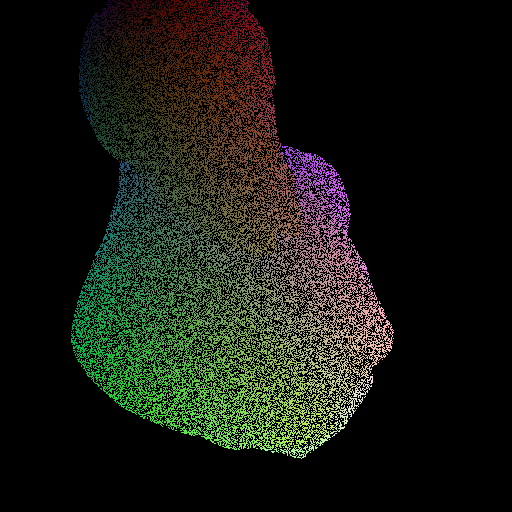
\includegraphics[width=.2\textwidth]{./pic/00440.vertex.png}};
	\node[text width=3.5cm] at (\vdist*\disttimes,\yschift-1.5) {3D Vertex};

	\draw [-stealth](\vdist*\disttimes,\yschift-1.5) -- (\vdist*\disttimes,\yschift-1.7);

	\draw [-stealth]  (\vdist*\disttimes+2,\yschift) -- (\vdist*\disttimes+1.5,\yschift);

	\pgfmathsetmacro{\disttimes}{7}
	\pgfmathsetmacro{\yschift}{\preprocessingshift}
	\node[inner sep=0pt] (depthmap) at (\vdist*\disttimes,\yschift)
	{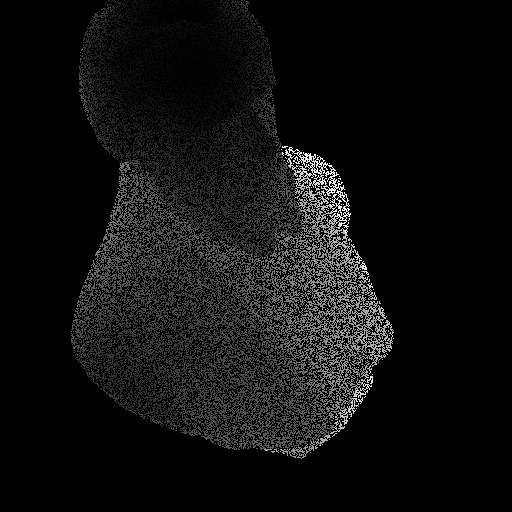
\includegraphics[width=.2\textwidth]{./pic/00440.depth0_noise.png}};
	\node[text width=3.5cm] at (\vdist*\disttimes,\yschift-1.5) {Depth Map + noise};


	\draw [-stealth] (\vdist*\disttimes+2,\yschift) -- (\vdist*\disttimes+1.5,\yschift);
	\pgfmathsetmacro{\disttimes}{12}
	\pgfmathsetmacro{\yschift}{\preprocessingshift}
	\node[inner sep=0pt] (depthmap) at (\vdist*\disttimes,\yschift)
	{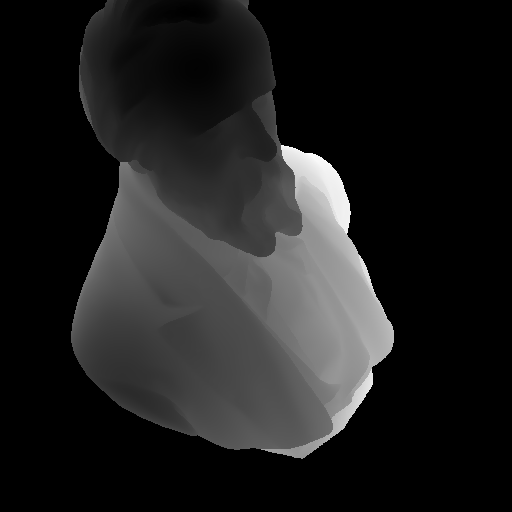
\includegraphics[width=.2\textwidth]{./pic/00440.depth0.png}};
	\node[text width=2cm] at (\vdist*\disttimes,\yschift-1.5) {Depth Map};


	%% ------------------------------------------- vertex input ----------------------------------------------
	%% 	d_in							3x512x512


	%%	dconv1: 	d_in-->x1 			32x512x512
	\pgfmathsetmacro{\disttimes}{1}	%% width 32
	\pgfmathsetmacro{\boxsize}{\boxsizea}	%% size 512
	\pgfmathsetmacro{\boxwidth}{\boxwidthb}	%% width 32
	\pgfmathsetmacro{\yschift}{\gconvwshift}
	\node[text width=1cm] at (\vdist*\disttimes+0.1,\yschift-3.5) {32};
	\draw[black, fill=gconvcolor] (\vdist*\disttimes,\yschift,0) -- ++(-\boxwidth,0,0) -- ++(0,-\boxsize,0) -- ++(\boxwidth,0,0) -- cycle;
	\draw[black, fill=gconvcolor] (\vdist*\disttimes,\yschift,0) -- ++(0,0,-\boxsize) -- ++(0,-\boxsize,0) -- ++(0,0,\boxsize) -- cycle;
	\draw[black, fill=gconvcolor] (\vdist*\disttimes,\yschift,0) -- ++(-\boxwidth,0,0) -- ++(0,0,-\boxsize) -- ++(\boxwidth,0,0) -- cycle;

	%%	dconv2:		x1-->x1				32x512x512
	\pgfmathsetmacro{\disttimes}{2}	%% width 32
	\pgfmathsetmacro{\boxsize}{\boxsizea}	%% size 512
	\pgfmathsetmacro{\boxwidth}{\boxwidthb}	%% width 32
	\pgfmathsetmacro{\yschift}{\gconvwshift}
	\draw[black, fill=gconvcolor] (\vdist*\disttimes,\yschift,0) -- ++(-\boxwidth,0,0) -- ++(0,-\boxsize,0) -- ++(\boxwidth,0,0) -- cycle;
	\draw[black, fill=gconvcolor] (\vdist*\disttimes,\yschift,0) -- ++(0,0,-\boxsize) -- ++(0,-\boxsize,0) -- ++(0,0,\boxsize) -- cycle;
	\draw[black, fill=gconvcolor] (\vdist*\disttimes,\yschift,0) -- ++(-\boxwidth,0,0) -- ++(0,0,-\boxsize) -- ++(\boxwidth,0,0) -- cycle;

	%%	dconv3:		x1-->x1				32x512x512
	\pgfmathsetmacro{\disttimes}{3}	%% width 32
	\pgfmathsetmacro{\boxsize}{\boxsizea}	%% size 512
	\pgfmathsetmacro{\boxwidth}{\boxwidthb}	%% width 32
	\pgfmathsetmacro{\yschift}{\gconvwshift}
	\draw[black, fill=gconvcolor] (\vdist*\disttimes,\yschift,0) -- ++(-\boxwidth,0,0) -- ++(0,-\boxsize,0) -- ++(\boxwidth,0,0) -- cycle;
	\draw[black, fill=gconvcolor] (\vdist*\disttimes,\yschift,0) -- ++(0,0,-\boxsize) -- ++(0,-\boxsize,0) -- ++(0,0,\boxsize) -- cycle;
	\draw[black, fill=gconvcolor] (\vdist*\disttimes,\yschift,0) -- ++(-\boxwidth,0,0) -- ++(0,0,-\boxsize) -- ++(\boxwidth,0,0) -- cycle;

	\draw (\vdist*\disttimes-0.2,\yschift-3.2) -- (\vdist*\disttimes-0.2,\yschift-4);
	\draw (\vdist*\disttimes-0.2,\yschift-4) -- (\vdist*\disttimes+5.7,\yschift-4);
	\draw [-stealth] (\vdist*\disttimes+5.7,\yschift-4) -- (\vdist*\disttimes+5.7,\yschift-5.2);
	%% downsample 1
	%%	dconv4:		x1-->x2				32x256x256
	\pgfmathsetmacro{\disttimes}{4}	%% width 32
	\pgfmathsetmacro{\boxsize}{\boxsizeb}	%% size 256
	\pgfmathsetmacro{\boxwidth}{\boxwidthb}	%% width 32
	\pgfmathsetmacro{\yschift}{\gconvwshift-0.5}	%% width 32
	\draw[black, fill=gconvcolor] (\vdist*\disttimes,\yschift,0) -- ++(-\boxwidth,0,0) -- ++(0,-\boxsize,0) -- ++(\boxwidth,0,0) -- cycle;
	\draw[black, fill=gconvcolor] (\vdist*\disttimes,\yschift,0) -- ++(0,0,-\boxsize) -- ++(0,-\boxsize,0) -- ++(0,0,\boxsize) -- cycle;
	\draw[black, fill=gconvcolor] (\vdist*\disttimes,\yschift,0) -- ++(-\boxwidth,0,0) -- ++(0,0,-\boxsize) -- ++(\boxwidth,0,0) -- cycle;
	%%	dconv2:		x2-->x2				32x256x256
	\pgfmathsetmacro{\disttimes}{5}	%% width 32
	\pgfmathsetmacro{\boxsize}{\boxsizeb}	%% size 256
	\pgfmathsetmacro{\boxwidth}{\boxwidthb}	%% width 32
	\pgfmathsetmacro{\yschift}{\gconvwshift-0.5}	%% width 32
	\draw[black, fill=gconvcolor] (\vdist*\disttimes,\yschift,0) -- ++(-\boxwidth,0,0) -- ++(0,-\boxsize,0) -- ++(\boxwidth,0,0) -- cycle;
	\draw[black, fill=gconvcolor] (\vdist*\disttimes,\yschift,0) -- ++(0,0,-\boxsize) -- ++(0,-\boxsize,0) -- ++(0,0,\boxsize) -- cycle;
	\draw[black, fill=gconvcolor] (\vdist*\disttimes,\yschift,0) -- ++(-\boxwidth,0,0) -- ++(0,0,-\boxsize) -- ++(\boxwidth,0,0) -- cycle;
	%%	dconv3:		x2-->x2				32x256x256
	\pgfmathsetmacro{\disttimes}{6}	%% width 32
	\pgfmathsetmacro{\boxsize}{\boxsizeb}	%% size 256
	\pgfmathsetmacro{\boxwidth}{\boxwidthb}	%% width 32
	\pgfmathsetmacro{\yschift}{\gconvwshift-0.5}	%% width 32
	\draw[black, fill=gconvcolor] (\vdist*\disttimes,\yschift,0) -- ++(-\boxwidth,0,0) -- ++(0,-\boxsize,0) -- ++(\boxwidth,0,0) -- cycle;
	\draw[black, fill=gconvcolor] (\vdist*\disttimes,\yschift,0) -- ++(0,0,-\boxsize) -- ++(0,-\boxsize,0) -- ++(0,0,\boxsize) -- cycle;
	\draw[black, fill=gconvcolor] (\vdist*\disttimes,\yschift,0) -- ++(-\boxwidth,0,0) -- ++(0,0,-\boxsize) -- ++(\boxwidth,0,0) -- cycle;

	\draw (\vdist*\disttimes-0.2,\yschift-1.6) -- (\vdist*\disttimes-0.2,\yschift-2.7);
	\draw (\vdist*\disttimes-0.2,\yschift-2.7) -- (\vdist*\disttimes+4.6,\yschift-2.7);
	\draw [-stealth] (\vdist*\disttimes+4.6,\yschift-2.7) -- (\vdist*\disttimes+4.6,\yschift-5.8);
	%% downsample 2
	%%	dconv4:		x2-->x3				32x128x128
	\pgfmathsetmacro{\disttimes}{7}	%% width 32
	\pgfmathsetmacro{\boxsize}{\boxsizec}	%% size 128
	\pgfmathsetmacro{\boxwidth}{\boxwidthb}	%% width 32
	\pgfmathsetmacro{\yschift}{\gconvwshift-0.8}	%% width 32
	\draw[black, fill=gconvcolor] (\vdist*\disttimes,\yschift,0) -- ++(-\boxwidth,0,0) -- ++(0,-\boxsize,0) -- ++(\boxwidth,0,0) -- cycle;
	\draw[black, fill=gconvcolor] (\vdist*\disttimes,\yschift,0) -- ++(0,0,-\boxsize) -- ++(0,-\boxsize,0) -- ++(0,0,\boxsize) -- cycle;
	\draw[black, fill=gconvcolor] (\vdist*\disttimes,\yschift,0) -- ++(-\boxwidth,0,0) -- ++(0,0,-\boxsize) -- ++(\boxwidth,0,0) -- cycle;
	%%	dconv2:		x3-->x3				32x128x128
	\pgfmathsetmacro{\disttimes}{8}	%% width 32
	\pgfmathsetmacro{\boxsize}{\boxsizec}	%% size 128
	\pgfmathsetmacro{\boxwidth}{\boxwidthb}	%% width 32
	\pgfmathsetmacro{\yschift}{\gconvwshift-0.8}	%% width 32
	\draw[black, fill=gconvcolor] (\vdist*\disttimes,\yschift,0) -- ++(-\boxwidth,0,0) -- ++(0,-\boxsize,0) -- ++(\boxwidth,0,0) -- cycle;
	\draw[black, fill=gconvcolor] (\vdist*\disttimes,\yschift,0) -- ++(0,0,-\boxsize) -- ++(0,-\boxsize,0) -- ++(0,0,\boxsize) -- cycle;
	\draw[black, fill=gconvcolor] (\vdist*\disttimes,\yschift,0) -- ++(-\boxwidth,0,0) -- ++(0,0,-\boxsize) -- ++(\boxwidth,0,0) -- cycle;
	%%	dconv3:		x3-->x3				32x128x128
	\pgfmathsetmacro{\disttimes}{9}	%% width 32
	\pgfmathsetmacro{\boxsize}{\boxsizec}	%% size 128
	\pgfmathsetmacro{\boxwidth}{\boxwidthb}	%% width 32
	\pgfmathsetmacro{\yschift}{\gconvwshift-0.8}	%% width 32
	\draw[black, fill=gconvcolor] (\vdist*\disttimes,\yschift,0) -- ++(-\boxwidth,0,0) -- ++(0,-\boxsize,0) -- ++(\boxwidth,0,0) -- cycle;
	\draw[black, fill=gconvcolor] (\vdist*\disttimes,\yschift,0) -- ++(0,0,-\boxsize) -- ++(0,-\boxsize,0) -- ++(0,0,\boxsize) -- cycle;
	\draw[black, fill=gconvcolor] (\vdist*\disttimes,\yschift,0) -- ++(-\boxwidth,0,0) -- ++(0,0,-\boxsize) -- ++(\boxwidth,0,0) -- cycle;
	%% downsample 3
	%%	dconv4:		x3-->x4				32x64x64
	\pgfmathsetmacro{\disttimes}{10}
	\pgfmathsetmacro{\boxsize}{\boxsized}	%% size 64
	\pgfmathsetmacro{\boxwidth}{\boxwidthb}	%% width 32
	\pgfmathsetmacro{\yschift}{\gconvwshift-1}
	\draw[black, fill=gconvcolor] (\vdist*\disttimes,\yschift,0) -- ++(-\boxwidth,0,0) -- ++(0,-\boxsize,0) -- ++(\boxwidth,0,0) -- cycle;
	\draw[black, fill=gconvcolor] (\vdist*\disttimes,\yschift,0) -- ++(0,0,-\boxsize) -- ++(0,-\boxsize,0) -- ++(0,0,\boxsize) -- cycle;
	\draw[black, fill=gconvcolor] (\vdist*\disttimes,\yschift,0) -- ++(-\boxwidth,0,0) -- ++(0,0,-\boxsize) -- ++(\boxwidth,0,0) -- cycle;
	%%	dconv2:		x4-->x4				32x64x64
	\pgfmathsetmacro{\disttimes}{11}
	\pgfmathsetmacro{\boxsize}{\boxsized}	%% size 64
	\pgfmathsetmacro{\boxwidth}{\boxwidthb}	%% width 32
	\pgfmathsetmacro{\yschift}{\gconvwshift-1}	%% width 32
	\draw[black, fill=gconvcolor] (\vdist*\disttimes,\yschift,0) -- ++(-\boxwidth,0,0) -- ++(0,-\boxsize,0) -- ++(\boxwidth,0,0) -- cycle;
	\draw[black, fill=gconvcolor] (\vdist*\disttimes,\yschift,0) -- ++(0,0,-\boxsize) -- ++(0,-\boxsize,0) -- ++(0,0,\boxsize) -- cycle;
	\draw[black, fill=gconvcolor] (\vdist*\disttimes,\yschift,0) -- ++(-\boxwidth,0,0) -- ++(0,0,-\boxsize) -- ++(\boxwidth,0,0) -- cycle;
	%%	dconv3:		x4-->x4				32x64x64
	\pgfmathsetmacro{\disttimes}{12}
	\pgfmathsetmacro{\boxsize}{\boxsized}	%% size 64
	\pgfmathsetmacro{\boxwidth}{\boxwidthb}	%% width 32
	\pgfmathsetmacro{\yschift}{\gconvwshift-1}	%% width 32
	\draw[black, fill=gconvcolor] (\vdist*\disttimes,\yschift,0) -- ++(-\boxwidth,0,0) -- ++(0,-\boxsize,0) -- ++(\boxwidth,0,0) -- cycle;
	\draw[black, fill=gconvcolor] (\vdist*\disttimes,\yschift,0) -- ++(0,0,-\boxsize) -- ++(0,-\boxsize,0) -- ++(0,0,\boxsize) -- cycle;
	\draw[black, fill=gconvcolor] (\vdist*\disttimes,\yschift,0) -- ++(-\boxwidth,0,0) -- ++(0,0,-\boxsize) -- ++(\boxwidth,0,0) -- cycle;

	%% dilated
	%%	dilated1:	x4-->x4				32x64x64
	\pgfmathsetmacro{\disttimes}{13}
	\pgfmathsetmacro{\boxsize}{\boxsized}	%% size 64
	\pgfmathsetmacro{\boxwidth}{\boxwidthb}	%% width 32
	\pgfmathsetmacro{\yschift}{\gconvwshift-1}	%% width 32
	\draw[black, fill=gconvdilatedcolor] (\vdist*\disttimes,\yschift,0) -- ++(-\boxwidth,0,0) -- ++(0,-\boxsize,0) -- ++(\boxwidth,0,0) -- cycle;
	\draw[black, fill=gconvdilatedcolor] (\vdist*\disttimes,\yschift,0) -- ++(0,0,-\boxsize) -- ++(0,-\boxsize,0) -- ++(0,0,\boxsize) -- cycle;
	\draw[black, fill=gconvdilatedcolor] (\vdist*\disttimes,\yschift,0) -- ++(-\boxwidth,0,0) -- ++(0,0,-\boxsize) -- ++(\boxwidth,0,0) -- cycle;
	%%	dilated2:	x4-->x4				32x64x64
	\pgfmathsetmacro{\disttimes}{14}
	\pgfmathsetmacro{\boxsize}{\boxsized}	%% size 64
	\pgfmathsetmacro{\boxwidth}{\boxwidthb}	%% width 32
	\pgfmathsetmacro{\yschift}{\gconvwshift-1}	%% width 32
	\draw[black, fill=gconvdilatedcolor] (\vdist*\disttimes,\yschift,0) -- ++(-\boxwidth,0,0) -- ++(0,-\boxsize,0) -- ++(\boxwidth,0,0) -- cycle;
	\draw[black, fill=gconvdilatedcolor] (\vdist*\disttimes,\yschift,0) -- ++(0,0,-\boxsize) -- ++(0,-\boxsize,0) -- ++(0,0,\boxsize) -- cycle;
	\draw[black, fill=gconvdilatedcolor] (\vdist*\disttimes,\yschift,0) -- ++(-\boxwidth,0,0) -- ++(0,0,-\boxsize) -- ++(\boxwidth,0,0) -- cycle;
	%%	dilated3:	x4-->x4				32x64x64
	\pgfmathsetmacro{\disttimes}{15}
	\pgfmathsetmacro{\boxsize}{\boxsized}	%% size 64
	\pgfmathsetmacro{\boxwidth}{\boxwidthb}	%% width 32
	\pgfmathsetmacro{\yschift}{\gconvwshift-1}	%% width 32
	\draw[black, fill=gconvdilatedcolor] (\vdist*\disttimes,\yschift,0) -- ++(-\boxwidth,0,0) -- ++(0,-\boxsize,0) -- ++(\boxwidth,0,0) -- cycle;
	\draw[black, fill=gconvdilatedcolor] (\vdist*\disttimes,\yschift,0) -- ++(0,0,-\boxsize) -- ++(0,-\boxsize,0) -- ++(0,0,\boxsize) -- cycle;
	\draw[black, fill=gconvdilatedcolor] (\vdist*\disttimes,\yschift,0) -- ++(-\boxwidth,0,0) -- ++(0,0,-\boxsize) -- ++(\boxwidth,0,0) -- cycle;
	%%	dilated4:	x4-->x4				32x64x64
	\pgfmathsetmacro{\disttimes}{16}
	\pgfmathsetmacro{\boxsize}{\boxsized}	%% size 64
	\pgfmathsetmacro{\boxwidth}{\boxwidthb}	%% width 32
	\pgfmathsetmacro{\yschift}{\gconvwshift-1}	%% width 32
	\draw[black, fill=gconvdilatedcolor] (\vdist*\disttimes,\yschift,0) -- ++(-\boxwidth,0,0) -- ++(0,-\boxsize,0) -- ++(\boxwidth,0,0) -- cycle;
	\draw[black, fill=gconvdilatedcolor] (\vdist*\disttimes,\yschift,0) -- ++(0,0,-\boxsize) -- ++(0,-\boxsize,0) -- ++(0,0,\boxsize) -- cycle;
	\draw[black, fill=gconvdilatedcolor] (\vdist*\disttimes,\yschift,0) -- ++(-\boxwidth,0,0) -- ++(0,0,-\boxsize) -- ++(\boxwidth,0,0) -- cycle;
	%%	dconv2:		x4-->x4				32x64x64
	\pgfmathsetmacro{\disttimes}{17}
	\pgfmathsetmacro{\boxsize}{\boxsized}	%% size 64
	\pgfmathsetmacro{\boxwidth}{\boxwidthb}	%% width 32
	\pgfmathsetmacro{\yschift}{\gconvwshift-1}	%% width 32
	\draw[black, fill=gconvcolor] (\vdist*\disttimes,\yschift,0) -- ++(-\boxwidth,0,0) -- ++(0,-\boxsize,0) -- ++(\boxwidth,0,0) -- cycle;
	\draw[black, fill=gconvcolor] (\vdist*\disttimes,\yschift,0) -- ++(0,0,-\boxsize) -- ++(0,-\boxsize,0) -- ++(0,0,\boxsize) -- cycle;
	\draw[black, fill=gconvcolor] (\vdist*\disttimes,\yschift,0) -- ++(-\boxwidth,0,0) -- ++(0,0,-\boxsize) -- ++(\boxwidth,0,0) -- cycle;
	%%	dconv3:		x4-->x4				32x64x64
	\pgfmathsetmacro{\disttimes}{18}
	\pgfmathsetmacro{\boxsize}{\boxsized}	%% size 64
	\pgfmathsetmacro{\boxwidth}{\boxwidthb}	%% width 32
	\pgfmathsetmacro{\yschift}{\gconvwshift-1}	%% width 32
	\draw[black, fill=gconvcolor] (\vdist*\disttimes,\yschift,0) -- ++(-\boxwidth,0,0) -- ++(0,-\boxsize,0) -- ++(\boxwidth,0,0) -- cycle;
	\draw[black, fill=gconvcolor] (\vdist*\disttimes,\yschift,0) -- ++(0,0,-\boxsize) -- ++(0,-\boxsize,0) -- ++(0,0,\boxsize) -- cycle;
	\draw[black, fill=gconvcolor] (\vdist*\disttimes,\yschift,0) -- ++(-\boxwidth,0,0) -- ++(0,0,-\boxsize) -- ++(\boxwidth,0,0) -- cycle;

	\draw (\vdist*\disttimes+0.25,\yschift-0.25) -- (\catx,\yschift-0.25);
	\draw [-stealth](\catx,\yschift-0.25) -- (\catx,\caty);




	%% ------------------------------ img feature ----------------------------------------------------------------

	\pgfmathsetmacro{\disttimes}{0}
	\pgfmathsetmacro{\yschift}{\convwshift-1}
	\node[inner sep=0pt] (depthmap) at (\vdist*\disttimes,\yschift)
	{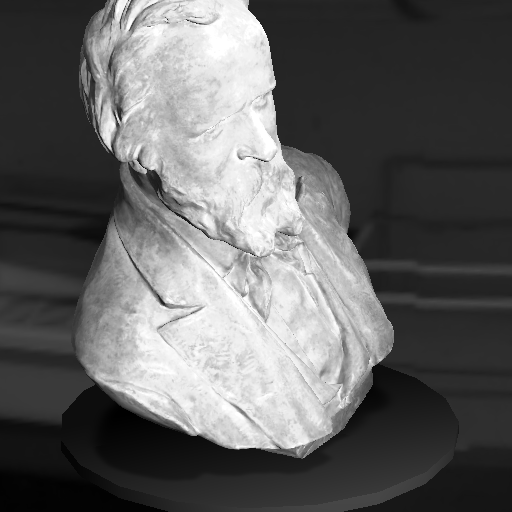
\includegraphics[width=.2\textwidth]{./pic/00440.image0.png}};
	\node[text width=3cm] at (\vdist*\disttimes,\yschift-1.5) {Gray Scale Image};
	\draw [-stealth](\vdist*\disttimes+1.5,\yschift) -- (\vdist*\disttimes+2.5,\yschift);

	%%	img_conv1:	img_in-->x_img_1 	32x512x512
	\pgfmathsetmacro{\disttimes}{\convrowstart + 1}
	\pgfmathsetmacro{\boxsize}{\boxsizea}	%% size 512
	\pgfmathsetmacro{\boxwidth}{\boxwidthb}	%% width 32
	\pgfmathsetmacro{\yschift}{\convwshift}
	\draw[black, fill=convcolor] (\vdist*\disttimes,\yschift,0) -- ++(-\boxwidth,0,0) -- ++(0,-\boxsize,0) -- ++(\boxwidth,0,0) -- cycle;
	\draw[black, fill=convcolor] (\vdist*\disttimes,\yschift,0) -- ++(0,0,-\boxsize) -- ++(0,-\boxsize,0) -- ++(0,0,\boxsize) -- cycle;
	\draw[black, fill=convcolor] (\vdist*\disttimes,\yschift,0) -- ++(-\boxwidth,0,0) -- ++(0,0,-\boxsize) -- ++(\boxwidth,0,0) -- cycle;
	%%	img_conv2:	x_img_1-->x_img_1	32x512x512
	\pgfmathsetmacro{\disttimes}{\convrowstart+2}	%% width 32
	\pgfmathsetmacro{\boxsize}{\boxsizea}	%% size 512
	\pgfmathsetmacro{\boxwidth}{\boxwidthb}	%% width 32
	\pgfmathsetmacro{\yschift}{\convwshift}
	\draw[black, fill=convcolor] (\vdist*\disttimes,\yschift,0) -- ++(-\boxwidth,0,0) -- ++(0,-\boxsize,0) -- ++(\boxwidth,0,0) -- cycle;
	\draw[black, fill=convcolor] (\vdist*\disttimes,\yschift,0) -- ++(0,0,-\boxsize) -- ++(0,-\boxsize,0) -- ++(0,0,\boxsize) -- cycle;
	\draw[black, fill=convcolor] (\vdist*\disttimes,\yschift,0) -- ++(-\boxwidth,0,0) -- ++(0,0,-\boxsize) -- ++(\boxwidth,0,0) -- cycle;
	%%	img_conv3:	x_img_1-->x_img_1	32x512x512
	\pgfmathsetmacro{\disttimes}{\convrowstart+3}	%% width 32
	\pgfmathsetmacro{\boxsize}{\boxsizea}	%% size 256
	\pgfmathsetmacro{\boxwidth}{\boxwidthb}	%% width 32
	\pgfmathsetmacro{\yschift}{\convwshift}
	\draw[black, fill=convcolor] (\vdist*\disttimes,\yschift,0) -- ++(-\boxwidth,0,0) -- ++(0,-\boxsize,0) -- ++(\boxwidth,0,0) -- cycle;
	\draw[black, fill=convcolor] (\vdist*\disttimes,\yschift,0) -- ++(0,0,-\boxsize) -- ++(0,-\boxsize,0) -- ++(0,0,\boxsize) -- cycle;
	\draw[black, fill=convcolor] (\vdist*\disttimes,\yschift,0) -- ++(-\boxwidth,0,0) -- ++(0,0,-\boxsize) -- ++(\boxwidth,0,0) -- cycle;

	%% downsample 1
	%%	img_conv4:	x_img_1-->x_img_2 	32x256x256
	\pgfmathsetmacro{\disttimes}{\convrowstart+4}
	\pgfmathsetmacro{\boxsize}{\boxsizeb}	%% size 256
	\pgfmathsetmacro{\boxwidth}{\boxwidthb}	%% width 32
	\pgfmathsetmacro{\yschift}{\convwshift-0.5}
	\draw[black, fill=convcolor] (\vdist*\disttimes,\yschift,0) -- ++(-\boxwidth,0,0) -- ++(0,-\boxsize,0) -- ++(\boxwidth,0,0) -- cycle;
	\draw[black, fill=convcolor] (\vdist*\disttimes,\yschift,0) -- ++(0,0,-\boxsize) -- ++(0,-\boxsize,0) -- ++(0,0,\boxsize) -- cycle;
	\draw[black, fill=convcolor] (\vdist*\disttimes,\yschift,0) -- ++(-\boxwidth,0,0) -- ++(0,0,-\boxsize) -- ++(\boxwidth,0,0) -- cycle;
	%%	img_conv2:	x_img_2-->x_img_2	32x256x256
	\pgfmathsetmacro{\disttimes}{\convrowstart+5}
	\pgfmathsetmacro{\boxsize}{\boxsizeb}	%% size 256
	\pgfmathsetmacro{\boxwidth}{\boxwidthb}	%% width 32
	\pgfmathsetmacro{\yschift}{\convwshift-.5}
	\draw[black, fill=convcolor] (\vdist*\disttimes,\yschift,0) -- ++(-\boxwidth,0,0) -- ++(0,-\boxsize,0) -- ++(\boxwidth,0,0) -- cycle;
	\draw[black, fill=convcolor] (\vdist*\disttimes,\yschift,0) -- ++(0,0,-\boxsize) -- ++(0,-\boxsize,0) -- ++(0,0,\boxsize) -- cycle;
	\draw[black, fill=convcolor] (\vdist*\disttimes,\yschift,0) -- ++(-\boxwidth,0,0) -- ++(0,0,-\boxsize) -- ++(\boxwidth,0,0) -- cycle;
	%%	img_conv3:	x_img_2-->x_img_2	32x256x256
	\pgfmathsetmacro{\disttimes}{\convrowstart+6}
	\pgfmathsetmacro{\boxsize}{\boxsizeb}	%% size 256
	\pgfmathsetmacro{\boxwidth}{\boxwidthb}	%% width 32
	\pgfmathsetmacro{\yschift}{\convwshift-0.5}
	\draw[black, fill=convcolor] (\vdist*\disttimes,\yschift,0) -- ++(-\boxwidth,0,0) -- ++(0,-\boxsize,0) -- ++(\boxwidth,0,0) -- cycle;
	\draw[black, fill=convcolor] (\vdist*\disttimes,\yschift,0) -- ++(0,0,-\boxsize) -- ++(0,-\boxsize,0) -- ++(0,0,\boxsize) -- cycle;
	\draw[black, fill=convcolor] (\vdist*\disttimes,\yschift,0) -- ++(-\boxwidth,0,0) -- ++(0,0,-\boxsize) -- ++(\boxwidth,0,0) -- cycle;

	%% downsample 2
	%%	img_conv4:	x_img_2-->x_img_3 	32x128x128
	\pgfmathsetmacro{\disttimes}{\convrowstart+7}
	\pgfmathsetmacro{\boxsize}{\boxsizec}	%% size 128
	\pgfmathsetmacro{\boxwidth}{\boxwidthb}	%% width 32
	\pgfmathsetmacro{\yschift}{\convwshift-1}
	\draw[black, fill=convcolor] (\vdist*\disttimes,\yschift,0) -- ++(-\boxwidth,0,0) -- ++(0,-\boxsize,0) -- ++(\boxwidth,0,0) -- cycle;
	\draw[black, fill=convcolor] (\vdist*\disttimes,\yschift,0) -- ++(0,0,-\boxsize) -- ++(0,-\boxsize,0) -- ++(0,0,\boxsize) -- cycle;
	\draw[black, fill=convcolor] (\vdist*\disttimes,\yschift,0) -- ++(-\boxwidth,0,0) -- ++(0,0,-\boxsize) -- ++(\boxwidth,0,0) -- cycle;
	%%	img_conv2:	x_img_3-->x_img_3	32x128x128
	\pgfmathsetmacro{\disttimes}{\convrowstart+8}
	\pgfmathsetmacro{\boxsize}{\boxsizec}	%% size 128
	\pgfmathsetmacro{\boxwidth}{\boxwidthb}	%% width 32
	\pgfmathsetmacro{\yschift}{\convwshift-1}
	\draw[black, fill=convcolor] (\vdist*\disttimes,\yschift,0) -- ++(-\boxwidth,0,0) -- ++(0,-\boxsize,0) -- ++(\boxwidth,0,0) -- cycle;
	\draw[black, fill=convcolor] (\vdist*\disttimes,\yschift,0) -- ++(0,0,-\boxsize) -- ++(0,-\boxsize,0) -- ++(0,0,\boxsize) -- cycle;
	\draw[black, fill=convcolor] (\vdist*\disttimes,\yschift,0) -- ++(-\boxwidth,0,0) -- ++(0,0,-\boxsize) -- ++(\boxwidth,0,0) -- cycle;
	%%	img_conv3:	x_img_3-->x_img_3	32x128x128
	\pgfmathsetmacro{\disttimes}{\convrowstart+9}
	\pgfmathsetmacro{\boxsize}{\boxsizec}	%% size 128
	\pgfmathsetmacro{\boxwidth}{\boxwidthb}	%% width 32
	\pgfmathsetmacro{\yschift}{\convwshift-1}
	\draw[black, fill=convcolor] (\vdist*\disttimes,\yschift,0) -- ++(-\boxwidth,0,0) -- ++(0,-\boxsize,0) -- ++(\boxwidth,0,0) -- cycle;
	\draw[black, fill=convcolor] (\vdist*\disttimes,\yschift,0) -- ++(0,0,-\boxsize) -- ++(0,-\boxsize,0) -- ++(0,0,\boxsize) -- cycle;
	\draw[black, fill=convcolor] (\vdist*\disttimes,\yschift,0) -- ++(-\boxwidth,0,0) -- ++(0,0,-\boxsize) -- ++(\boxwidth,0,0) -- cycle;

	%% downsample 3
	%%	img_conv4:	x_img_3-->x_img_4 	32x64x64
	\pgfmathsetmacro{\disttimes}{\convrowstart+10}
	\pgfmathsetmacro{\boxsize}{\boxsized}	%% size 64
	\pgfmathsetmacro{\boxwidth}{\boxwidthb}	%% width 32
	\pgfmathsetmacro{\yschift}{\convwshift-1.25}
	\draw[black, fill=convcolor] (\vdist*\disttimes,\yschift,0) -- ++(-\boxwidth,0,0) -- ++(0,-\boxsize,0) -- ++(\boxwidth,0,0) -- cycle;
	\draw[black, fill=convcolor] (\vdist*\disttimes,\yschift,0) -- ++(0,0,-\boxsize) -- ++(0,-\boxsize,0) -- ++(0,0,\boxsize) -- cycle;
	\draw[black, fill=convcolor] (\vdist*\disttimes,\yschift,0) -- ++(-\boxwidth,0,0) -- ++(0,0,-\boxsize) -- ++(\boxwidth,0,0) -- cycle;
	%%	img_conv2:	x_img_4-->x_img_4	32x64x64
	\pgfmathsetmacro{\disttimes}{\convrowstart+11}
	\pgfmathsetmacro{\boxsize}{\boxsized}	%% size 64
	\pgfmathsetmacro{\boxwidth}{\boxwidthb}	%% width 32
	\pgfmathsetmacro{\yschift}{\convwshift-1.25}
	\draw[black, fill=convcolor] (\vdist*\disttimes,\yschift,0) -- ++(-\boxwidth,0,0) -- ++(0,-\boxsize,0) -- ++(\boxwidth,0,0) -- cycle;
	\draw[black, fill=convcolor] (\vdist*\disttimes,\yschift,0) -- ++(0,0,-\boxsize) -- ++(0,-\boxsize,0) -- ++(0,0,\boxsize) -- cycle;
	\draw[black, fill=convcolor] (\vdist*\disttimes,\yschift,0) -- ++(-\boxwidth,0,0) -- ++(0,0,-\boxsize) -- ++(\boxwidth,0,0) -- cycle;
	%%	img_conv3:	x_img_4-->x_img_4	32x64x64
	\pgfmathsetmacro{\disttimes}{\convrowstart+12}
	\pgfmathsetmacro{\boxsize}{\boxsized}	%% size 64
	\pgfmathsetmacro{\boxwidth}{\boxwidthb}	%% width 32
	\pgfmathsetmacro{\yschift}{\convwshift-1.25}
	\draw[black, fill=convcolor] (\vdist*\disttimes,\yschift,0) -- ++(-\boxwidth,0,0) -- ++(0,-\boxsize,0) -- ++(\boxwidth,0,0) -- cycle;
	\draw[black, fill=convcolor] (\vdist*\disttimes,\yschift,0) -- ++(0,0,-\boxsize) -- ++(0,-\boxsize,0) -- ++(0,0,\boxsize) -- cycle;
	\draw[black, fill=convcolor] (\vdist*\disttimes,\yschift,0) -- ++(-\boxwidth,0,0) -- ++(0,0,-\boxsize) -- ++(\boxwidth,0,0) -- cycle;


	\draw (\vdist*\disttimes+0.25,\yschift-0.25) -- (\catx+\boxwidth,\yschift-0.25);
	\draw [-stealth](\catx+\boxwidth,\yschift-0.25) -- (\catx+\boxwidth,\caty);

	%% ----------------------------------------- merge ------------------------------------------------------------------------------
	%%			x4,x_img_4-->x4			64x64x64

	\pgfmathsetmacro{\disttimes}{20}
	%% x4
	\pgfmathsetmacro{\boxsize}{\boxsized}	%% size 64
	\pgfmathsetmacro{\boxwidth}{\boxwidthb}	%% width 32
	\pgfmathsetmacro{\yschift}{\caty}
	\draw[black, fill=gconvcolor] (\catx,\yschift,0) -- ++(-\boxwidth,0,0) -- ++(0,-\boxsize,0) -- ++(\boxwidth,0,0) -- cycle;
	\draw[black, fill=gconvcolor] (\catx,\yschift,0) -- ++(0,0,-\boxsize) -- ++(0,-\boxsize,0) -- ++(0,0,\boxsize) -- cycle;
	\draw[black, fill=gconvcolor] (\catx,\yschift,0) -- ++(-\boxwidth,0,0) -- ++(0,0,-\boxsize) -- ++(\boxwidth,0,0) -- cycle;
	%% x_img_4
	\pgfmathsetmacro{\boxsize}{\boxsized}	%% size 64
	\pgfmathsetmacro{\boxwidth}{\boxwidthb}	%% width 32
	\pgfmathsetmacro{\yschift}{\caty}	%% width 32
	\draw[black, fill=convcolor] (\catx+\boxwidth,\yschift,0) -- ++(-\boxwidth,0,0) -- ++(0,-\boxsize,0) -- ++(\boxwidth,0,0) -- cycle;
	\draw[black, fill=convcolor] (\catx+\boxwidth,\yschift,0) -- ++(0,0,-\boxsize) -- ++(0,-\boxsize,0) -- ++(0,0,\boxsize) -- cycle;
	\draw[black, fill=convcolor] (\catx+\boxwidth,\yschift,0) -- ++(-\boxwidth,0,0) -- ++(0,0,-\boxsize) -- ++(\boxwidth,0,0) -- cycle;


	\node[text width=1cm] at (\catx,\caty-1) {concatenate};


	%% --------------------------------------------- output normal map --------------------------------------------------------------------
	\pgfmathsetmacro{\disttimes}{2.3}
	\pgfmathsetmacro{\yschift}{\secrowshift-0.5}
	\node[inner sep=0pt] (depthmap) at (\vdist*\disttimes,\yschift)
	{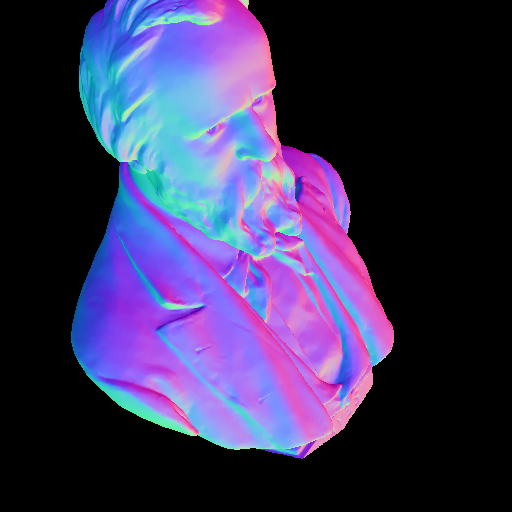
\includegraphics[width=.2\textwidth]{./pic/00440.normal0.png}};
	\node[text width=2cm] at (\vdist*\disttimes,\yschift-1.5) {Normal Map};

	\draw [-stealth] (\vdist*\disttimes+2.5,\yschift) -- (\vdist*\disttimes+2,\yschift);


	%% ------------------------------------- output ----------------------------------------------------------------------------------------
	%% conv2		xout-->xout			3x512x512
	\pgfmathsetmacro{\disttimes}{\secondrowstart + 3}
	\pgfmathsetmacro{\boxsize}{\boxsizea}	%% size 512
	\pgfmathsetmacro{\boxwidth}{\boxwidtha}	%% width 3
	\pgfmathsetmacro{\yschift}{\secrowshift+0.5}	%% width 32
	\draw[black, fill=convcolor] (\vdist*\disttimes,\yschift,0) -- ++(-\boxwidth,0,0) -- ++(0,-\boxsize,0) -- ++(\boxwidth,0,0) -- cycle;
	\draw[black, fill=convcolor] (\vdist*\disttimes,\yschift,0) -- ++(0,0,-\boxsize) -- ++(0,-\boxsize,0) -- ++(0,0,\boxsize) -- cycle;
	\draw[black, fill=convcolor] (\vdist*\disttimes,\yschift,0) -- ++(-\boxwidth,0,0) -- ++(0,0,-\boxsize) -- ++(\boxwidth,0,0) -- cycle;


	%% conv1		x1-->xout			3x512x512
	\pgfmathsetmacro{\disttimes}{\secondrowstart + 4}
	\pgfmathsetmacro{\boxsize}{\boxsizea}	%% size 512
	\pgfmathsetmacro{\boxwidth}{\boxwidtha}	%% width 3
	\pgfmathsetmacro{\yschift}{\secrowshift+0.5}	%% width 32
	\node[text width=1cm] at (\vdist*\disttimes+0.4,\yschift-2.2) {3};
	\draw[black, fill=convcolor] (\vdist*\disttimes,\yschift,0) -- ++(-\boxwidth,0,0) -- ++(0,-\boxsize,0) -- ++(\boxwidth,0,0) -- cycle;
	\draw[black, fill=convcolor] (\vdist*\disttimes,\yschift,0) -- ++(0,0,-\boxsize) -- ++(0,-\boxsize,0) -- ++(0,0,\boxsize) -- cycle;
	\draw[black, fill=convcolor] (\vdist*\disttimes,\yschift,0) -- ++(-\boxwidth,0,0) -- ++(0,0,-\boxsize) -- ++(\boxwidth,0,0) -- cycle;


	%% ----------------------------------------------------------------------------------------------------------------------
	%% uconv3		x1,x1_us-->x1		32x512x512
	\pgfmathsetmacro{\disttimes}{\secondrowstart + 5}
	\pgfmathsetmacro{\boxsize}{\boxsizea}	%% size 512
	\pgfmathsetmacro{\boxwidth}{\boxwidthb}	%% width 32
	\pgfmathsetmacro{\yschift}{\secrowshift+0.5}	%% width 32
	\draw[black, fill=gconvcolor] (\vdist*\disttimes,\yschift,0) -- ++(-\boxwidth,0,0) -- ++(0,-\boxsize,0) -- ++(\boxwidth,0,0) -- cycle;
	\draw[black, fill=gconvcolor] (\vdist*\disttimes,\yschift,0) -- ++(0,0,-\boxsize) -- ++(0,-\boxsize,0) -- ++(0,0,\boxsize) -- cycle;
	\draw[black, fill=gconvcolor] (\vdist*\disttimes,\yschift,0) -- ++(-\boxwidth,0,0) -- ++(0,0,-\boxsize) -- ++(\boxwidth,0,0) -- cycle;

	%% upsample 3
	%% interpolate	x2-->x1_us			32x512x512
	\pgfmathsetmacro{\disttimes}{\secondrowstart + 6}
	\pgfmathsetmacro{\boxsize}{\boxsizea}	%% size 512
	\pgfmathsetmacro{\boxwidth}{\boxwidthb}	%% width 32
	\pgfmathsetmacro{\yschift}{\secrowshift+0.5}	%% width 32
	\draw[black, fill=gconvcolor] (\vdist*\disttimes,\yschift,0) -- ++(-\boxwidth,0,0) -- ++(0,-\boxsize,0) -- ++(\boxwidth,0,0) -- cycle;
	\draw[black, fill=gconvcolor] (\vdist*\disttimes,\yschift,0) -- ++(0,0,-\boxsize) -- ++(0,-\boxsize,0) -- ++(0,0,\boxsize) -- cycle;
	\draw[black, fill=gconvcolor] (\vdist*\disttimes,\yschift,0) -- ++(-\boxwidth,0,0) -- ++(0,0,-\boxsize) -- ++(\boxwidth,0,0) -- cycle;
	\pgfmathsetmacro{\boxsize}{\boxsizea}	%% size 512
	\pgfmathsetmacro{\boxwidth}{\boxwidthb}	%% width 32
	\pgfmathsetmacro{\yschift}{\secrowshift+0.5}	%% width 32
	\draw[black, fill=gconvcolor] (\vdist*\disttimes+\boxwidth,\yschift,0) -- ++(-\boxwidth,0,0) -- ++(0,-\boxsize,0) -- ++(\boxwidth,0,0) -- cycle;
	\draw[black, fill=gconvcolor] (\vdist*\disttimes+\boxwidth,\yschift,0) -- ++(0,0,-\boxsize) -- ++(0,-\boxsize,0) -- ++(0,0,\boxsize) -- cycle;
	\draw[black, fill=gconvcolor] (\vdist*\disttimes+\boxwidth,\yschift,0) -- ++(-\boxwidth,0,0) -- ++(0,0,-\boxsize) -- ++(\boxwidth,0,0) -- cycle;

	%% uconv2		x2,x2_us-->x2		32x256x256
	\pgfmathsetmacro{\disttimes}{\secondrowstart + 8}
	\pgfmathsetmacro{\boxsize}{\boxsizeb}	%% size 256
	\pgfmathsetmacro{\boxwidth}{\boxwidthb}	%% width 32
	\pgfmathsetmacro{\yschift}{\secrowshift}	%% width 32
	\draw[black, fill=gconvcolor] (\vdist*\disttimes,\yschift,0) -- ++(-\boxwidth,0,0) -- ++(0,-\boxsize,0) -- ++(\boxwidth,0,0) -- cycle;
	\draw[black, fill=gconvcolor] (\vdist*\disttimes,\yschift,0) -- ++(0,0,-\boxsize) -- ++(0,-\boxsize,0) -- ++(0,0,\boxsize) -- cycle;
	\draw[black, fill=gconvcolor] (\vdist*\disttimes,\yschift,0) -- ++(-\boxwidth,0,0) -- ++(0,0,-\boxsize) -- ++(\boxwidth,0,0) -- cycle;

	\pgfmathsetmacro{\boxsize}{\boxsizeb}	%% size 256
	\pgfmathsetmacro{\boxwidth}{\boxwidthb}	%% width 32
	\pgfmathsetmacro{\yschift}{\secrowshift}	%% width 32
	\draw[black, fill=gconvcolor] (\vdist*\disttimes+\boxwidth,\yschift,0) -- ++(-\boxwidth,0,0) -- ++(0,-\boxsize,0) -- ++(\boxwidth,0,0) -- cycle;
	\draw[black, fill=gconvcolor] (\vdist*\disttimes+\boxwidth,\yschift,0) -- ++(0,0,-\boxsize) -- ++(0,-\boxsize,0) -- ++(0,0,\boxsize) -- cycle;
	\draw[black, fill=gconvcolor] (\vdist*\disttimes+\boxwidth,\yschift,0) -- ++(-\boxwidth,0,0) -- ++(0,0,-\boxsize) -- ++(\boxwidth,0,0) -- cycle;

	%% upsample 2
	%% interpolate	x3-->x2_us			32x256x256
	\pgfmathsetmacro{\disttimes}{\secondrowstart + 10}
	\pgfmathsetmacro{\boxsize}{\boxsizeb}	%% size 256
	\pgfmathsetmacro{\boxwidth}{\boxwidthb}	%% width 32
	\pgfmathsetmacro{\yschift}{\secrowshift}	%% width 32
	\draw[black, fill=gconvcolor] (\vdist*\disttimes,\yschift,0) -- ++(-\boxwidth,0,0) -- ++(0,-\boxsize,0) -- ++(\boxwidth,0,0) -- cycle;
	\draw[black, fill=gconvcolor] (\vdist*\disttimes,\yschift,0) -- ++(0,0,-\boxsize) -- ++(0,-\boxsize,0) -- ++(0,0,\boxsize) -- cycle;
	\draw[black, fill=gconvcolor] (\vdist*\disttimes,\yschift,0) -- ++(-\boxwidth,0,0) -- ++(0,0,-\boxsize) -- ++(\boxwidth,0,0) -- cycle;

	%% uconv1		x3_us-->x3			32x128x128
	\pgfmathsetmacro{\disttimes}{\secondrowstart + 12}
	\pgfmathsetmacro{\boxsize}{\boxsizec}	%% size 128
	\pgfmathsetmacro{\boxwidth}{\boxwidthb}	%% width 32
	\pgfmathsetmacro{\yschift}{\secrowshift}	%% width 32
	\node[text width=1cm] at (\vdist*\disttimes+0.2,\yschift-1.5) {32};
	\draw[black, fill=gconvcolor] (\vdist*\disttimes,\yschift,0) -- ++(-\boxwidth,0,0) -- ++(0,-\boxsize,0) -- ++(\boxwidth,0,0) -- cycle;
	\draw[black, fill=gconvcolor] (\vdist*\disttimes,\yschift,0) -- ++(0,0,-\boxsize) -- ++(0,-\boxsize,0) -- ++(0,0,\boxsize) -- cycle;
	\draw[black, fill=gconvcolor] (\vdist*\disttimes,\yschift,0) -- ++(-\boxwidth,0,0) -- ++(0,0,-\boxsize) -- ++(\boxwidth,0,0) -- cycle;

	%% upsample 1
	%% interpolate	x4-->x3_us			64x128x128
	\pgfmathsetmacro{\disttimes}{\secondrowstart +14}
	\pgfmathsetmacro{\boxsize}{\boxsizec}	%% size 128
	\pgfmathsetmacro{\boxwidth}{\boxwidthc}	%% width 64
	\pgfmathsetmacro{\yschift}{\secrowshift}	%% width 32
	\node[text width=1cm] at (\vdist*\disttimes,\yschift-1.5) {64};
	\draw[black, fill=gconvcolor] (\vdist*\disttimes,\yschift,0) -- ++(-\boxwidth,0,0) -- ++(0,-\boxsize,0) -- ++(\boxwidth,0,0) -- cycle;
	\draw[black, fill=gconvcolor] (\vdist*\disttimes,\yschift,0) -- ++(0,0,-\boxsize) -- ++(0,-\boxsize,0) -- ++(0,0,\boxsize) -- cycle;
	\draw[black, fill=gconvcolor] (\vdist*\disttimes,\yschift,0) -- ++(-\boxwidth,0,0) -- ++(0,0,-\boxsize) -- ++(\boxwidth,0,0) -- cycle;

	\draw (\catx+0.3,\caty-1.3) -- (\catx+0.3,\secrowshift);
	\draw [-stealth] (\catx+0.3,\secrowshift) -- (\secondrowstart +9,\secrowshift);
\end{tikzpicture}

	\caption{CNN Architecture}
	\label{fig:cnn_archi}
\end{figure}










				


